\begin{figure}
	\centering
	\begin{subfigure}[b]{1\textwidth}
		\centering
		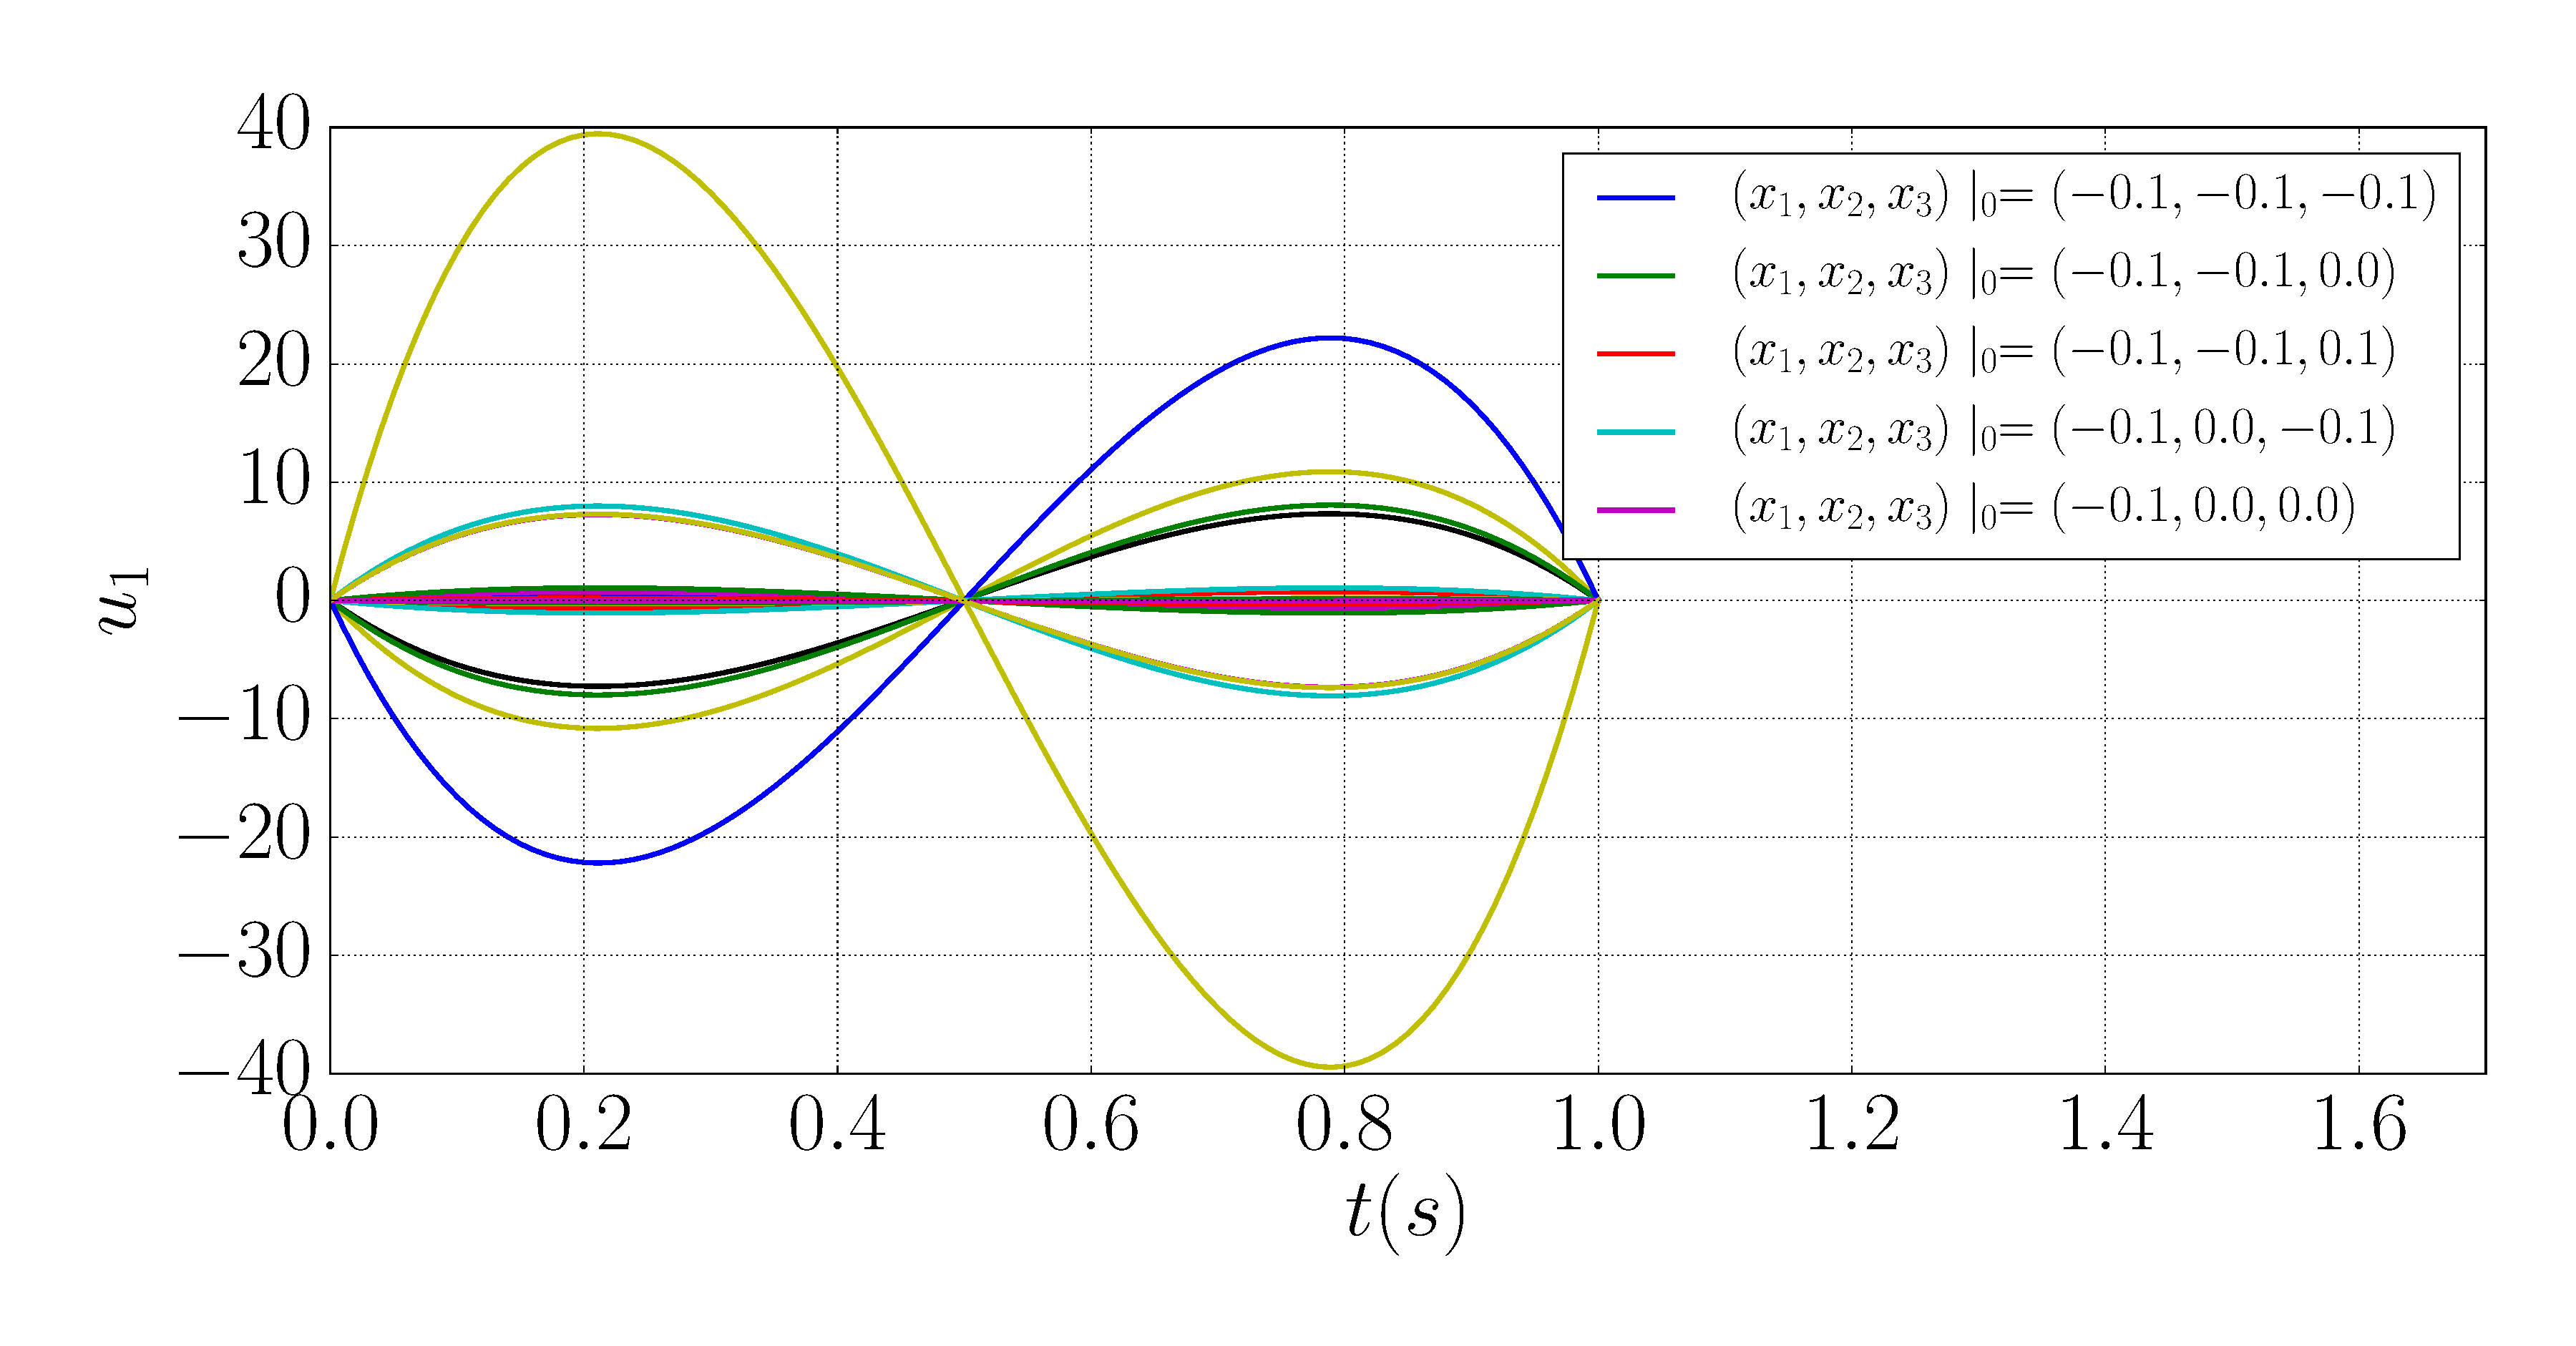
\includegraphics[width=15.5cm]{bild/30_32/Brockett_e2_Asy_Pytrajectory_d_01_u1.pdf}
		\label{fig:Trajektorien_von_u_1_aus_Pytrajectory}
		\caption{Trajektorien von $u_{1}$}
	\end{subfigure}%
	\hspace{1in} 
	\begin{subfigure}[b]{1\textwidth}
		\centering
		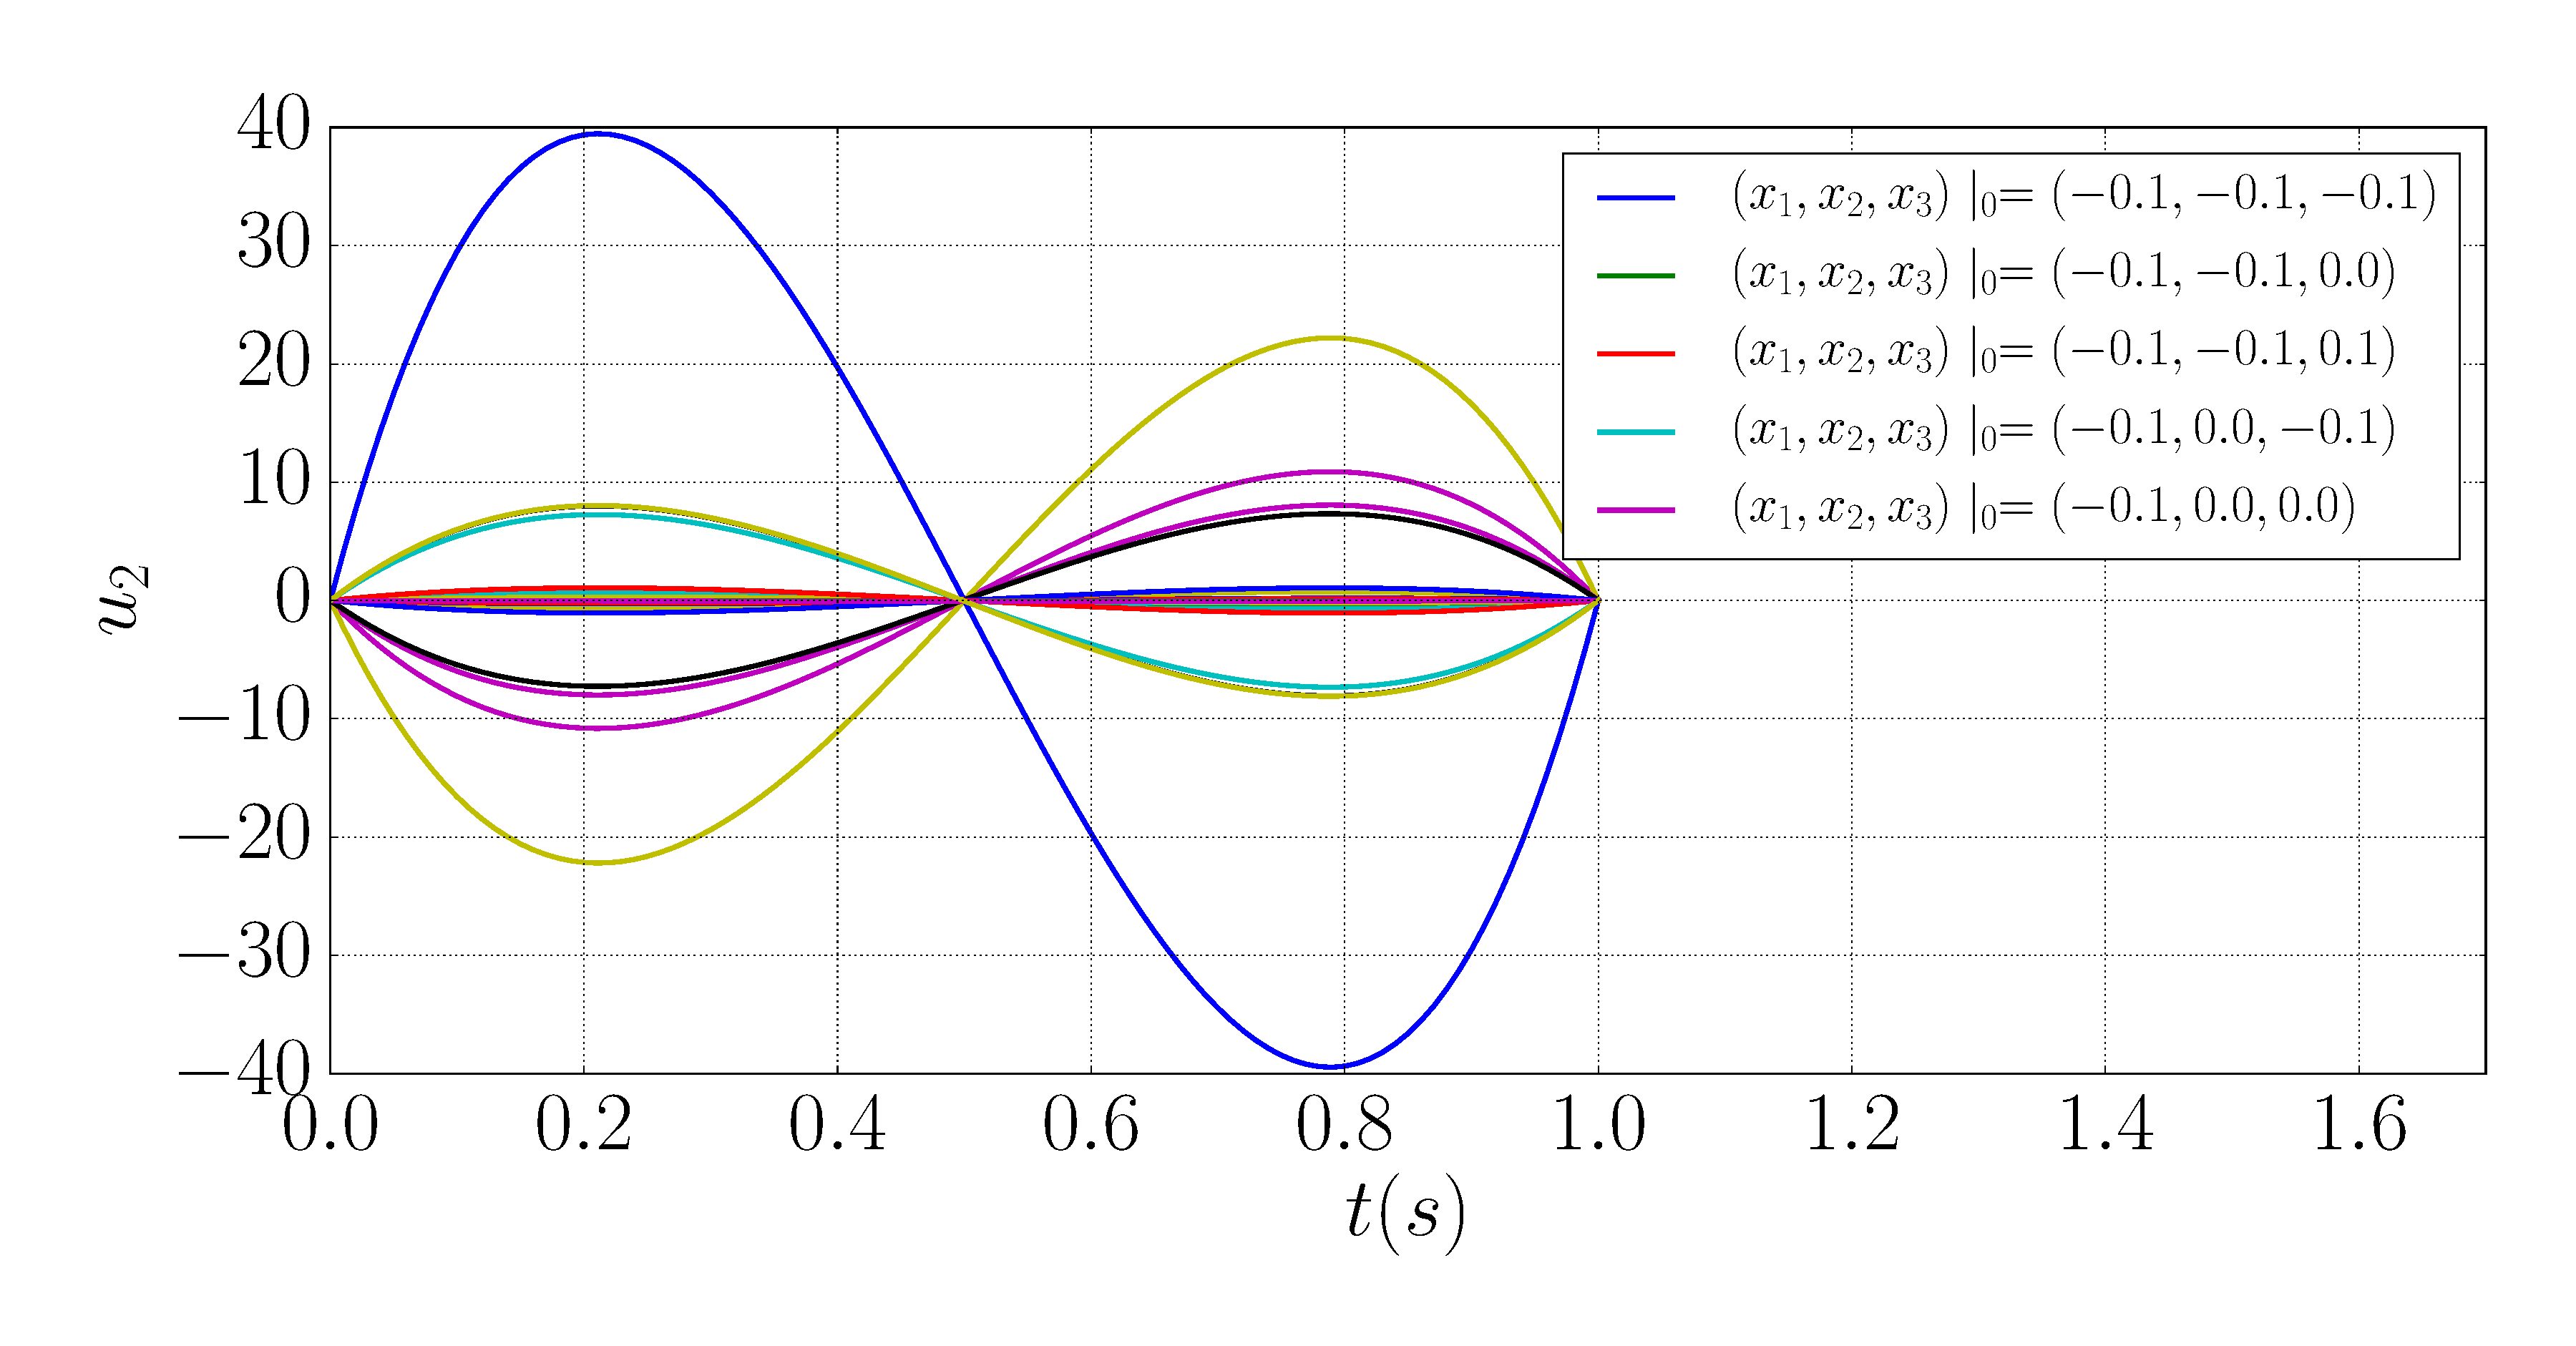
\includegraphics[width=15.5cm]{bild/30_32/Brockett_e2_Asy_Pytrajectory_d_01_u2.pdf}
		\label{fig:Trajektorien_von_u_2_aus_Pytrajectory}
		\caption{Trajektorien von $u_{2}$}
	\end{subfigure}
	\caption{Trajektorien der Systemeingänge mit verschiedenen $\vect{x}_{0}$ für den Brocketts nicht-holonimischen Doppelintegrator mittels \emph{Pytrajectory}.}
	\label{fig:Brocketts_Doppelintegrator_Asy_Pytr_ori}
\end{figure}